\documentclass{article}
\usepackage[margin=1in]{geometry}
\usepackage{amsmath,amsfonts}
\usepackage{parskip}
\usepackage{graphicx}
\usepackage{hyperref}
\setlength{\parindent}{0pt}

\begin{document}

\title{K-Square Project Onboarding Agent: Streamlining Execution Team Integration}
\author{Alberto Espinosa \\ KSquare Group}
\date{1 August 2025}
\maketitle

\begin{abstract}
The K-Square Project Onboarding Agent is an artificial intelligence system designed to streamline the onboarding process for programme execution teams following project acquisition. By automating the aggregation of internal and external data, the system enables teams to acquire domain knowledge, understand client contexts, and commence work efficiently. This paper presents the system’s architecture, core principles, implications, and relevance, with an evaluation of agentic technologies such as LangGraph and Ollama for implementation.
\end{abstract}

\section{Introduction}
The onboarding of programme execution teams after a project is won represents a critical phase in project management. Manual processes, which rely on gathering insights from sales, pre-sales, and other stakeholders, are time-consuming and prone to inefficiencies. The K-Square Project Onboarding Agent addresses this challenge by leveraging artificial intelligence to automate data aggregation and insight generation, enabling execution teams to integrate rapidly and effectively. This paper outlines the system’s design, its core ideas, and its potential impact on enterprise workflows.

\section{System Overview}
The K-Square Project Onboarding Agent is a closed-loop ecosystem that synthesises internal and external data to facilitate onboarding. It comprises three primary agents:
\begin{itemize}
    \item \textbf{Deep Dive Agent}: Conducts research by querying internal repositories (e.g., SharePoint) and the open web to gather client-specific and industry-relevant information. It employs human validation to ensure relevance.
    \item \textbf{Project Intelligence Agent}: Aggregates outputs from active agents to generate a dashboard of key insights, recommendations, and actionable outputs, such as summaries and statements of work.
    \item \textbf{Meetings Agent}: Analyses meeting data (e.g., transcripts, audio recordings) to extract action items, sentiment, and scope expansions, enhancing future interactions.
\end{itemize}
The system focuses on post-sales onboarding, relying on structured internal data (e.g., categorised SharePoint folders) to deliver domain knowledge, best practices, and client profiles within a condensed timeframe (2–3 days).

\subsection{System Workflow}
The system’s workflow is illustrated in Figure \ref{fig:overview}, which provides a high-level overview of data flow from client inputs to onboarding outputs. Client and project details are processed through data aggregation, agent analysis, and user validation, culminating in a dashboard that delivers actionable insights. This process ensures efficient integration of execution teams by automating repetitive tasks and leveraging structured data.

\begin{figure}[h]
    \centering
    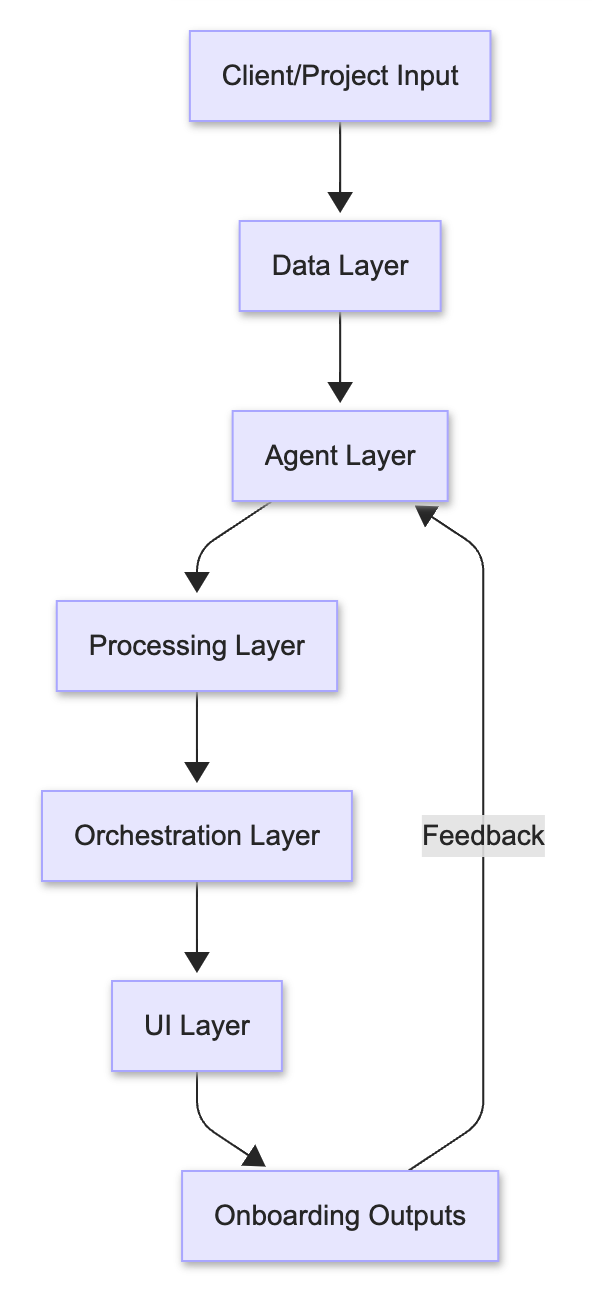
\includegraphics[width=0.3\textwidth]{/Users/albertohernandez/Documents/projects/KS-onboarding/doc/images/overview.png}
    \caption{High-level overview of the K-Square Project Onboarding Agent workflow.}
    \label{fig:overview}
\end{figure}

\section{Core Ideas}
The system is underpinned by several foundational principles:
\begin{itemize}
    \item \textbf{Automation}: By automating data aggregation and insight generation, the system reduces reliance on manual stakeholder interactions.
    \item \textbf{Human-in-the-Loop}: Users validate agent outputs to train the system, ensuring continuous improvement in accuracy and relevance.
    \item \textbf{Structured Data Reliance}: The system leverages well-organised internal repositories to enhance data retrieval and processing efficiency.
    \item \textbf{Actionable Outputs}: The system generates summaries, onboarding plans, and reusable templates to enable rapid project initiation.
\end{itemize}

\section{Implications}
The K-Square Project Onboarding Agent offers significant implications for programme management:
\begin{itemize}
    \item \textbf{Efficiency Gains}: Automation reduces onboarding time from weeks to days, enabling faster project execution.
    \item \textbf{Scalability}: The modular agentic architecture supports expansion to accommodate additional functionalities or larger datasets.
    \item \textbf{Enterprise Adoption}: Integration with existing tools (e.g., Microsoft Teams, SharePoint) aligns with enterprise workflows, facilitating adoption.
\end{itemize}

\section{Relevance}
The system addresses a critical need in programme management: the rapid integration of execution teams. By streamlining onboarding, it reduces dependency on stakeholder availability and ensures consistent delivery of domain knowledge. Its focus on post-sales execution aligns with enterprise priorities, making it a valuable tool for organisations seeking to optimise project initiation processes.

\section{Architectural Possibilities}
The system’s architecture can be realised using agentic technologies, with LangGraph and Ollama as primary candidates.

\subsection{LangGraph}
LangGraph, a graph-based framework for multi-agent workflows, is well-suited for orchestrating the system’s agents. It enables dynamic task routing, where outputs from the Deep Dive Agent feed the Project Intelligence Agent, ensuring efficient data flow. Its strengths include flexibility and context retention, which are critical for complex agent interactions. However, its complexity requires experienced developers, and simpler alternatives like CrewAI may be preferable for rapid prototyping.

\subsection{Ollama}
Ollama facilitates local deployment of large language models (e.g., LLaMA 3), ensuring data privacy and reducing cloud costs. It is ideal for processing sensitive internal data, such as SharePoint documents. However, its reliance on smaller models limits performance for large-scale inference, necessitating cloud-based alternatives (e.g., OpenAI) for external data processing. Combining Ollama with a cloud LLM offers a balanced approach.

\subsection{Alternatives}
CrewAI provides a simpler framework for agent collaboration, suitable for initial prototypes. Hugging Face Transformers supports fine-tuning for domain-specific tasks, enhancing accuracy. Pinecone or Weaviate can manage vector search for efficient document retrieval. A hybrid architecture, with LangGraph for orchestration, Ollama for internal processing, and cloud LLMs for external data, is recommended to optimise performance and privacy.

\section{Suggested Additional Features}
The Meetings Agent, as described in the System Overview, employs sentiment analysis to extract insights from meeting data, providing a valuable indication of the general tone and opinions expressed during client interactions. To enhance this capability, a novel approach proposed by \textbf{Alberto Espinosa} (\cite{espinosa2025}) in a recent scientific study introduces a formal dynamical measurement of opinion change based on semantics and complexity. This research, available at \href{https://arxiv.org/abs/2505.02581}{https://arxiv.org/abs/2505.02581}, develops a change-of-opinion attack test using perturbation and intervention analysis to study how conversational dynamics evolve. By tracking shifts in semantics, sentiment, and topics, this measurement offers a more granular understanding of meeting interactions, enabling the Meetings Agent to identify nuanced changes in client perspectives and adapt onboarding outputs accordingly. Integrating this approach would enhance the system’s ability to deliver precise, context-aware insights, aligning with the goal of streamlining execution team integration. 

This feature is a suggestion and is subject to evaluation and approval, as it involves a high-level mathematical implementation.


\section{Conclusion}
The K-Square Project Onboarding Agent represents a transformative solution for programme execution team integration. By automating onboarding through a robust agentic system, it delivers efficiency, scalability, and enterprise alignment. LangGraph and Ollama, complemented by alternative technologies, provide a feasible architectural foundation. Future work should focus on fine-tuning models, refining human-in-the-loop mechanisms, and incorporating advanced measurements of conversational dynamics to enhance system performance.

\begin{thebibliography}{1}
\bibitem{espinosa2025}
A. Espinosa, ``Embracing Inevitable AI Misalignment as a Strategy to Steer Competitive Agents Towards Human Alignment: Change-of-Opinion Attacks and Interventions,'' arXiv preprint arXiv:2505.02581, 2025.
\end{thebibliography}


\end{document}